\documentclass[10pt,a4paper,openany]{article}
\usepackage[latin1]{inputenc}
\usepackage[english]{babel}
\usepackage{amsmath}
\usepackage{amsfonts}
\usepackage{amssymb}
\usepackage{graphicx}
\usepackage{listings}
\usepackage{color}
\usepackage[left=2cm,right=1cm,top=3cm,bottom=2cm]{geometry}
\usepackage[numbers,sort&compress]{natbib}
\usepackage{url}
\usepackage{caption}
\usepackage{siunitx}
\usepackage{subfigure}
\usepackage{float}
\usepackage{booktabs}

\usepackage{comment}

\setlength{\parindent}{0pt}

\definecolor{mygreen}{rgb}{0,0.6,0}
\definecolor{mygray}{rgb}{0.5,0.5,0.5}
\definecolor{mymauve}{rgb}{0.58,0,0.82}

\lstset{ 
	backgroundcolor=\color{white},   % choose the background color; you must add \usepackage{color} or \usepackage{xcolor}; should come as last argument
	basicstyle=\footnotesize,        % the size of the fonts that are used for the code
	breakatwhitespace=false,         % sets if automatic breaks should only happen at whitespace
	breaklines=true,                 % sets automatic line breaking
	captionpos=b,                    % sets the caption-position to bottom
	commentstyle=\color{mygreen},    % comment style
	deletekeywords={...},            % if you want to delete keywords from the given language
	escapeinside={\%*}{*)},          % if you want to add LaTeX within your code
	extendedchars=true,              % lets you use non-ASCII characters; for 8-bits encodings only, does not work with UTF-8
	firstnumber=01,                	 % start line enumeration with line 1000
	frame=single,	                 % adds a frame around the code
	keepspaces=true,                 % keeps spaces in text, useful for keeping indentation of code (possibly needs columns=flexible)
	keywordstyle=\color{blue},       % keyword style
	language=Python,                 % the language of the code
	morekeywords={*,...},            % if you want to add more keywords to the set
	numbers=left,                    % where to put the line-numbers; possible values are (none, left, right)
	numbersep=5pt,                   % how far the line-numbers are from the code
	numberstyle=\tiny\color{mygray}, % the style that is used for the line-numbers
	rulecolor=\color{black},         % if not set, the frame-color may be changed on line-breaks within not-black text (e.g. comments (green here))
	showspaces=false,                % show spaces everywhere adding particular underscores; it overrides 'showstringspaces'
	showstringspaces=false,          % underline spaces within strings only
	showtabs=false,                  % show tabs within strings adding particular underscores
	stepnumber=1,                    % the step between two line-numbers. If it's 1, each line will be numbered
	stringstyle=\color{mymauve},     % string literal style
	tabsize=2,	                     % sets default tabsize to 2 spaces
	title=\lstname                   % show the filename of files included with \lstinputlisting; also try caption instead of title
}

\usepackage{titling}
\newcommand{\subtitle}[1]{%
	\posttitle{%
		\par\end{center}
	\begin{center}\large#1\end{center}
	\vskip0.5em}%
}


\author{5273}
\title{Homework Assignment 1: Applied Probabilistic Models}
\subtitle{Data Analysis of Growth Domestic Product category}
\date{}



\begin{document}
	
\maketitle

	\section*{Introduction}
	
	For this work, data is collected on the official website of Instituto Nacional de Estad�stica y Geograf�a (INEGI) \citep{inegi_data}. The chosen section is Growth Domestic Product, and within this section, a national macroeconomic indicator is selected: Global Index of Economic Activity (IGAE) for the data analysis. Data obtained from INEGI website are in \texttt{csv} format, edited in order to work with the general values of the three main representative activities each month, which the aforementioned indicator is based on. The objective is to evaluate the behavior of the group of activities and which has a major impact on the IGAE.
	
	For the analysis it is used the R software in its version 4.0.2 \citep{r} and the code used is available on the GitHub repository of  \citep{github}. This work is run on a MacBook Air with an Intel Core i5 CPU $ @ $ 1.8 GHz and 8 GB RAM.
	
	\section*{Data}
	\subsection*{Global Index of Economic Activity}
	 
	The IGAE  is an index that aproximates the calculation of the generated wealth in the country monthly. It is considered a trend index and marks the path that the national economic activity is reporting in the given month \citep{mvs}.
	It is important to emphasize that the IGAE collects monthly figures since January 1993.

	\subsection*{Calculation Methods}
	
	The method used to calculate the IGAE consists of monthly indexes of the physical volume of production for each of the selected classes, with a fixed base in 2013 \citep{calculo_igae}.
	
	The calculation of the physical volume index of industrial activities consists of preparing monthly indexes of the volume of real production for each of the classes that have information on quantities produced, production values, and prices at the product level.
	
	In general, an index number is the percentage relationship that measures the change from one time to another in price, quantity, value, or some other element of interest, and can be constructed for different periods, ranging from high frequency (daily, weekly, monthly, quarterly, etc.) to annual.
	
	In the case of  IGAE physical volume of production indexes are elaborated, of Laspeyres-type (an index that systematically overvalues inflation), as well as simple indexes based on a related indicator, expressed base 2013 = 100.
	
	\subsubsection*{Physical Volume Index of production, Laspeyres-type}
	
\begin{equation*}
	Q_{0,n}=\dfrac{\displaystyle\sum_{}^{} P_{0}Q_{n}}{\sum_{}^{} P_{0}Q_{0}/12}*100
\end{equation*}

Where:

	$Q_{0,n}$ = Physical volume index of the production of period $ n $ in relation to period $ 0 $.
	
	$0$ = base year.
	
	$ n $ = period of reference.
	
	$Q_{n}$ = Quantity of a produced good during period $ n $ (period of study).
	
	$Q_{0}$ = Quantity of a produced good during period $ 0 $ (base).
	
	$P_{0}$ = price of a good corresponding to the base period.
	
	
	\subsubsection*{Real value indexes (income or expenses)}
	
	\begin{equation*}
		IV =\dfrac{ I_{n}}{ I_{0}}*100
	\end{equation*}
	
	Where:
	
	$IV$ = Value index
	
	$I_{n}$ = Real income/expenses of study period
	
	$I_{0}$ = Real income/expenses of base period
	
	
	In the calculation of the IGAE, three fundamental areas or activities are involved: primary, secondary, and tertiary, which are detailed below.
	
	\subsubsection*{Primary Activities}
	
	These activities include agriculture, breeding, and exploitation of animals.
	
	
	\subsubsection*{Secondary Activities}
	
	These activities cover mining, generation, transmission, and distribution of electricity, water supply, and gas through pipelines to the final consumer, construction, and manufacturing industries.
	
	\subsubsection*{Tertiary Activities}
	
	This group of activities contains wholesale and retail; transport, post, and storage; media information; services such as financial and insurance, real state, rental and intangible property, professional, scientific, educational and technical services, business support and waste management, health and social assistance, recreational, cultural and sports services, temporary accommodation; legislative, governmental, justice administration and international activities.
	
	\section*{Representation and Analysis}
	
	For the data representation, it is selected data of 330 months starting from January 1993 to June 2020. A boxplot of the index values for each group of activities is represented in  Figure \ref{fig:box1}. Here the horizontal axis represents each of the group of activities and the vertical one represents the corresponding values of the index.
	
	\lstinputlisting[language=R, firstline=6, lastline=13]{t1.R}

	\begin{center}
		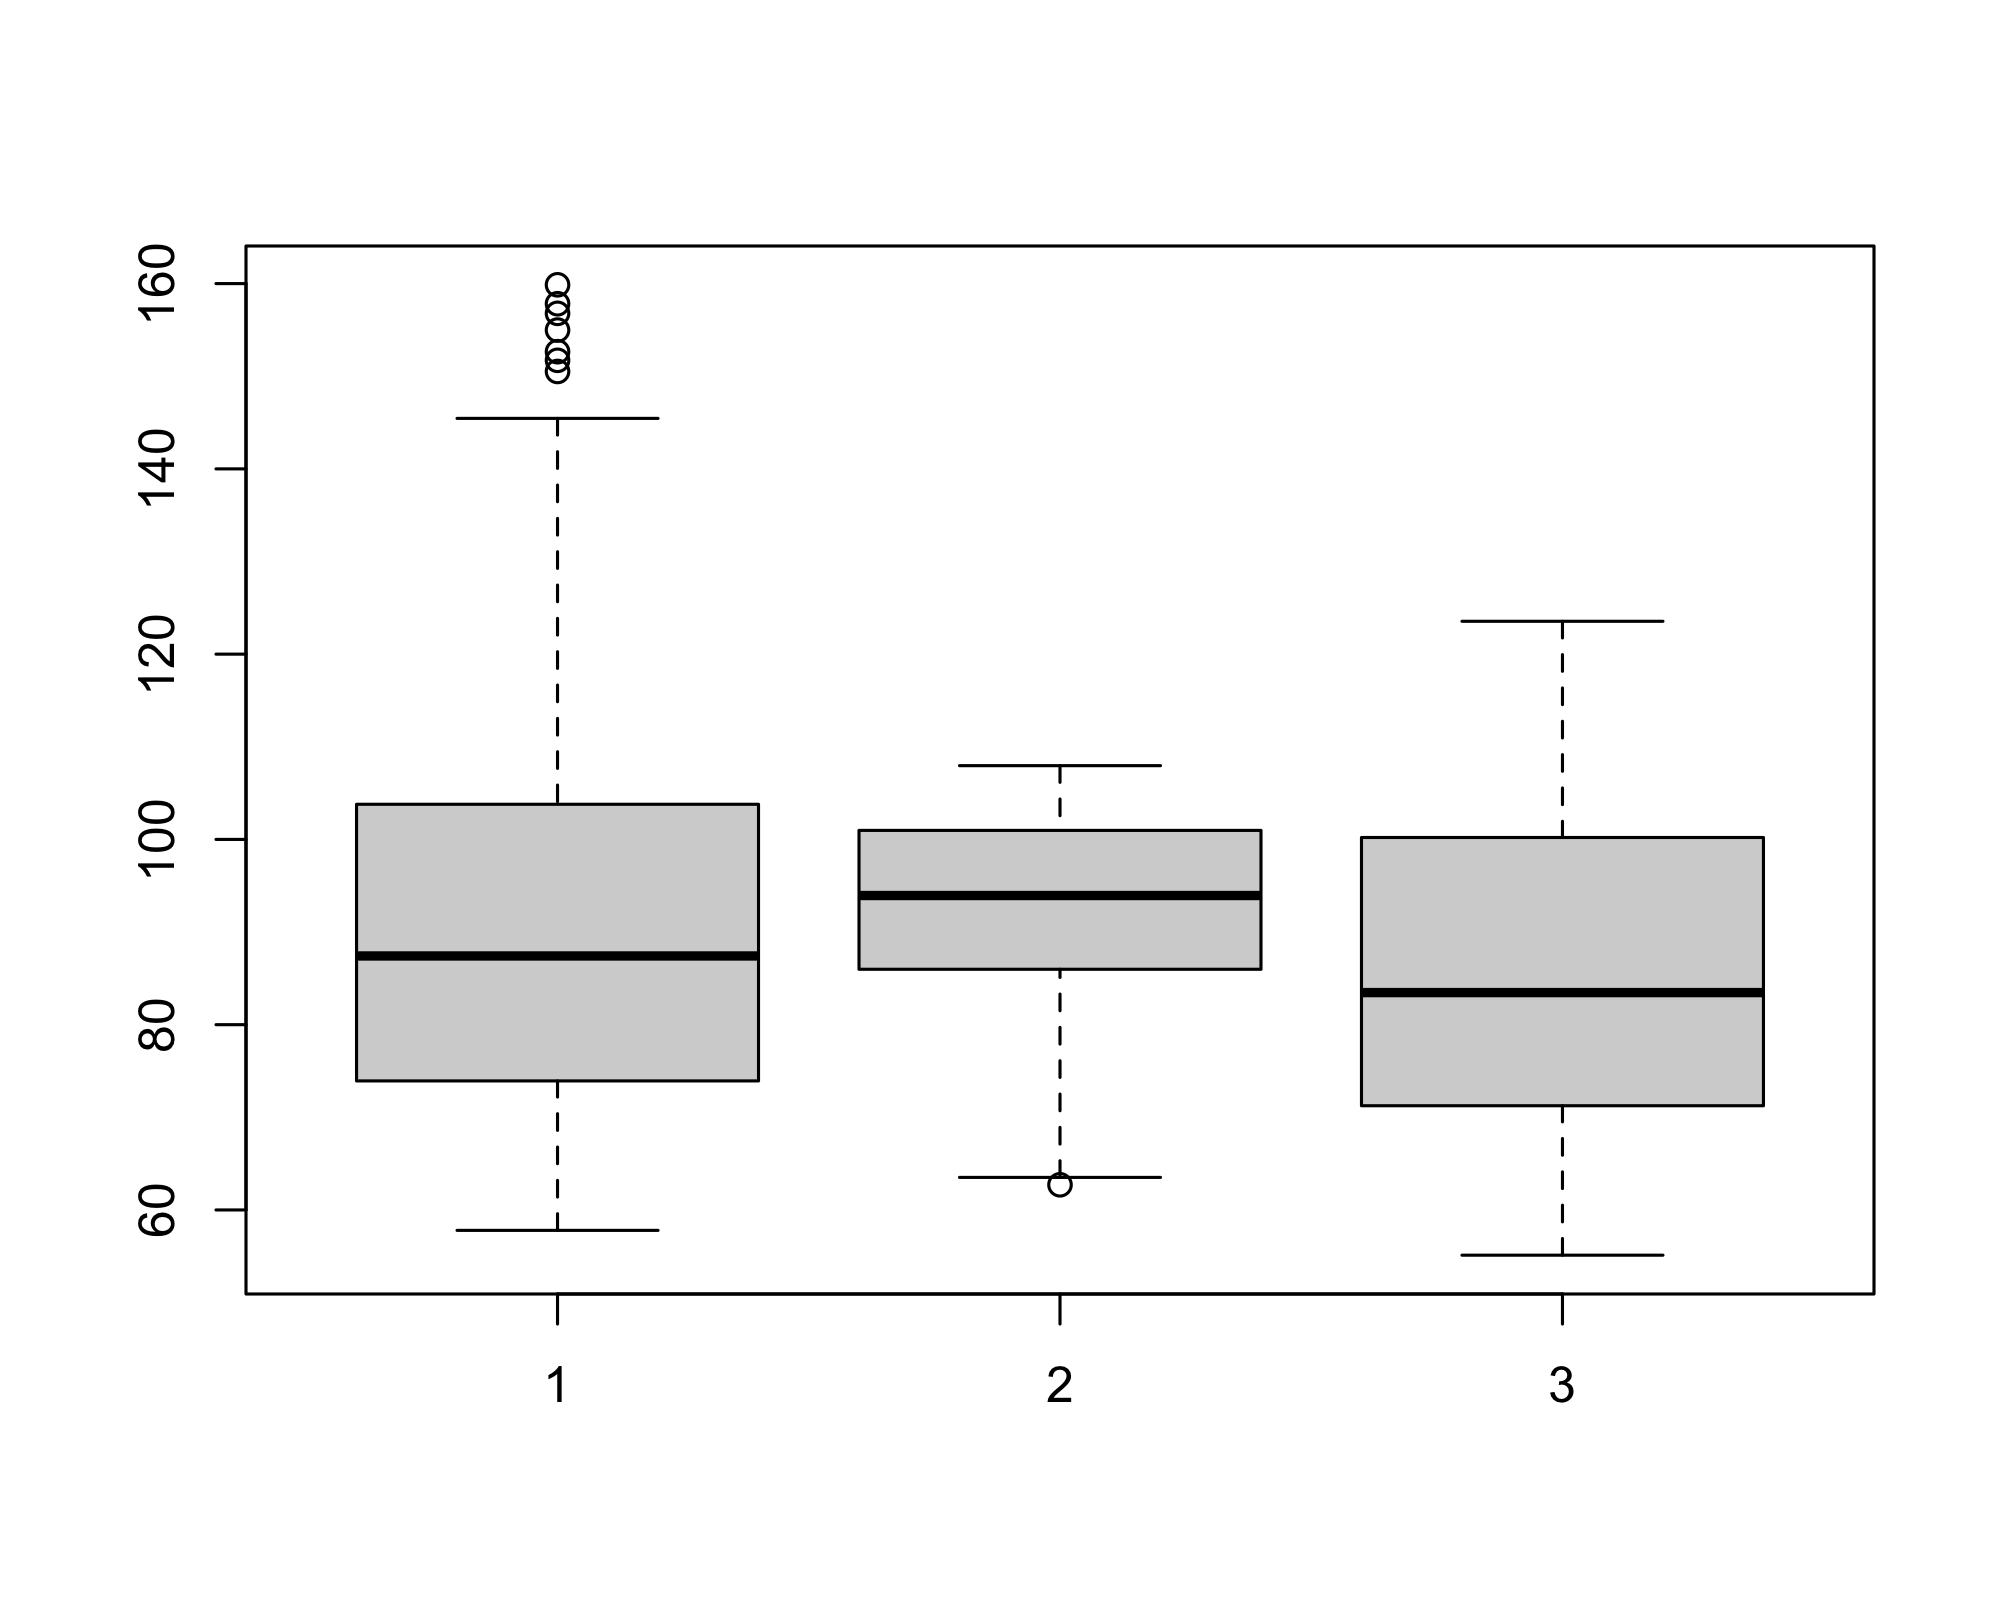
\includegraphics[scale=0.2]{boxplot_activities}
		\captionof{figure}{Boxplot of the three activities of the IGAE}
		\label{fig:box1}
	\end{center}

	After looking at the values of the three groups of activities it can be noticed a wider range of values in the primary activities. This primary activity also has higher values of the sample, with several outliers above the third quartile. The secondary activities are the least scattered so it the one that shows an overall performance over time. On the other hand, its higher values are not as great as primary and tertiary activities.
	
\newpage

	Primary activities can be analyzed further. In Figure \ref{fig:box2} it can be seen last two months of the year are months with higher action and August and September are the month with lower activity. Also in Figure \ref {fig:box3} it can be seen a growing trend with lows in the 19 and 26 boxes, as a consequence of the economic crisis of 2008 and COVID-19 respectively.  
	
	\begin{center}
		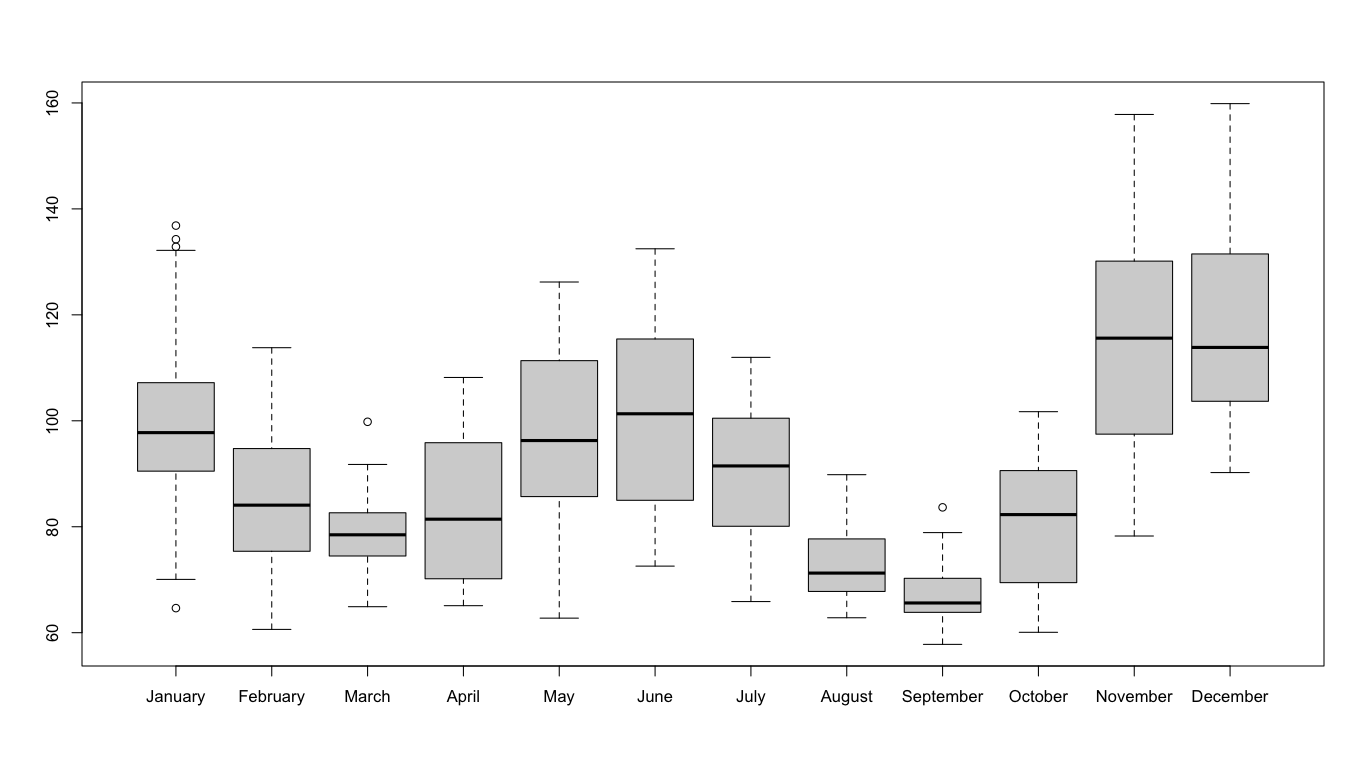
\includegraphics[scale=0.36]{boxplot_month1}
		\captionof{figure}{Boxplot of primary activities by months}
		\label{fig:box2}
	\end{center}

	\begin{center}
	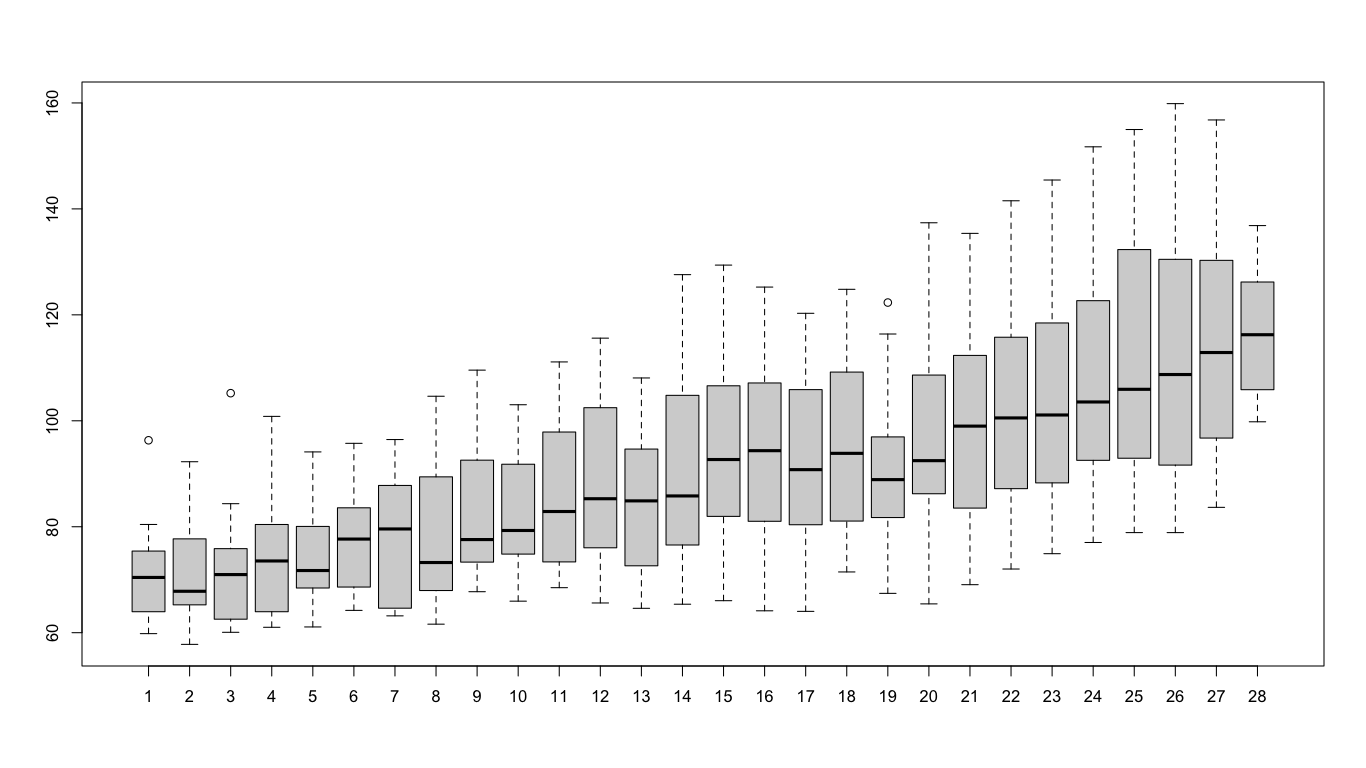
\includegraphics[scale=0.36]{boxplot_year1}
	\captionof{figure}{Boxplot of primary activites by year}
	\label{fig:box3}
\end{center}
	
	\bibliography{tarea1}
	\bibliographystyle{plainnat}
	
\end{document}